\section{Speed Optimization Experiments}

\subsection{Memory}
We first analyze the memory layout of the arrays used for calculation. Each
array element is of complex type double precision, occupying 16 bytes on a
64-bit GNU/Linux system.
\tiny\begin{verbatim}
    // C == std::complex

    sizeof(C<double>) == 16 bytes
    sizeof(double)    ==  8 bytes

    x0t0xtblock[2*NVEPLUS1]: 30 elements

    0         1         ...       14        15        ...
    +---------+---------+---------+---------+---------+---------+
    |C<double>|C<double>|   ...   |C<double>|C<double>|   ...   |
    |         |         |   ...   | R  |  I |         |   ...   |
    +---------+---------+---------+---------+---------+---------+
    ^                              ^               ^
    | x0t                          | t0            | xt
    | x0                             (double *)    | x1t1

    Hxt[NVEPLUS1*f::nve]: 15 * 14 == 210 elements

    0         1         ...       14        15        ...       196       ...
    +---------+---------+---------+---------+---------+---------+---------+---------+
    |C<double>|C<double>|   ...   |C<double>|C<double>|   ...   |C<double>|   ...   |
    |         |         |   ...   |         |         |   ...   |         |   ...   |
    +---------+---------+---------+---------+---------+---------+---------+---------+
    ^                                                           ^
    | HxH                                                       | RHS
    (const C<double> *const)
    dxdt[NVEPLUS1]: 15 elements

    0         1         ...       14        15
    +---------+---------+---------+---------+---------+
    |C<double>|C<double>|   ...   |C<double>|C<double>|
    |         |         |   ...   | R  |  I |         |
    +---------+---------+---------+---------+---------+
    ^                              ^
    | dx                           | dt
    | dx4                            (double *)

    dxi[f::nve]: 14 elements

    0         1         ...        14
    +---------+---------+---------+---------+
    |C<double>|C<double>|   ...   |C<double>|
    |         |         |   ...   |         |
    +---------+---------+---------+---------+

\end{verbatim}
\normalsize

By using a ``release with debug info'' build compiled under
\verb|GCC 7.5.0 x86_64-linux-gnu|, we can check the starting addresses of
each array with a debugger. By doing so, we find that there's a gap between,
\verb|x0t0xtblock| and \verb|Hxt| of 3264 bytes (204 elements).

Memory layout gap:
\footnotesize\begin{verbatim}

    MEMORY LAYOUT
    (range is inclusive: low <= x <= high):

    0x7fff f7a5 0000
          |
    +-----------+
    | 6100-61df | dxi
    +-----------+
    | 61e0-62cf | dxdt
    +-----------+
    | 62d0-64af | x0t0xtblock
    +-----------+
          |
      64b0-716f   GAP
          |
    +-----------+
    | 7170-7f2f | Hxt
    +-----------+
\end{verbatim}
\normalsize

\subsection{Valgrind}

Valgrind is a instrumentation framework and library of dynamic analysis tools.
By using Valgrind's capabilities, we can get further insight into the behavior
of the program during runtime.

We used Memcheck to first check for any possible memory leaks, but none were
found.

\begin{figure}[H]
    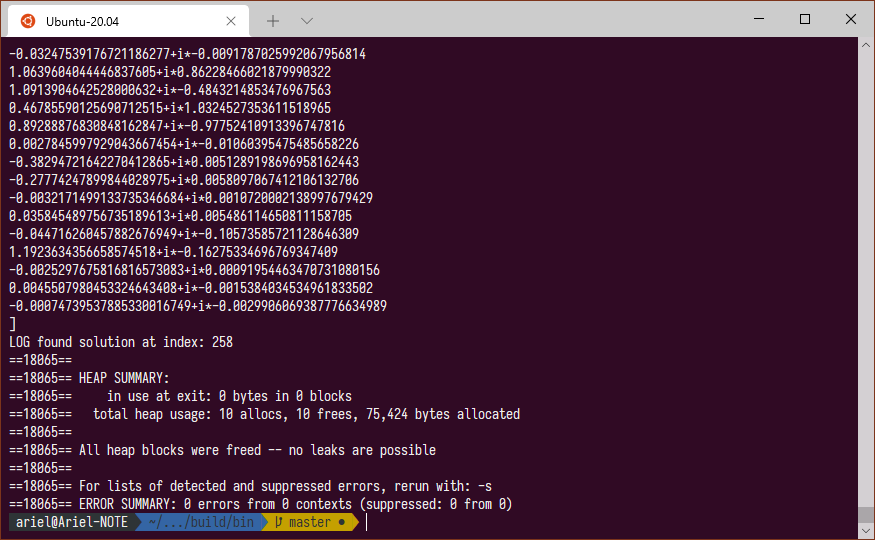
\includegraphics[width=\columnwidth]{figs/valgrind_memcheck}
    \caption{Valgrind Memcheck results}
\end{figure}

Next, we used Cachegrind to check for cache access, cache misses and branch
mispredictions, of which both were under 4\%.

\begin{figure}[H]
    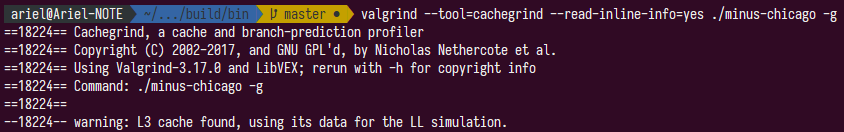
\includegraphics[width=\columnwidth]{figs/valgrind_cachegrind}
    \caption{Valgrind Cachegrind}
\end{figure}
\begin{figure}[H]
    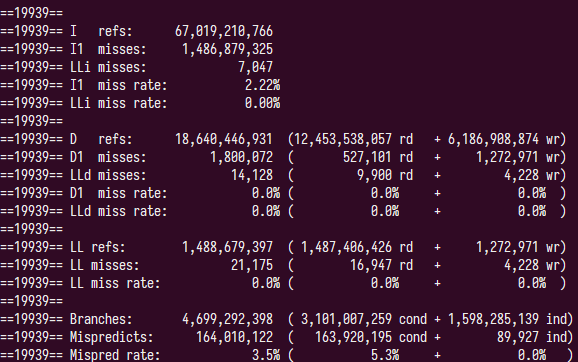
\includegraphics[width=\columnwidth]{figs/valgrind_cachegrind_results}
    \caption{Valgrind Cachegrind results}
\end{figure}

The tool Gg\_annotate allows for deeper understanding of the cache access
patterns which can be used to optimize memory access within functions.

\begin{figure}[H]
    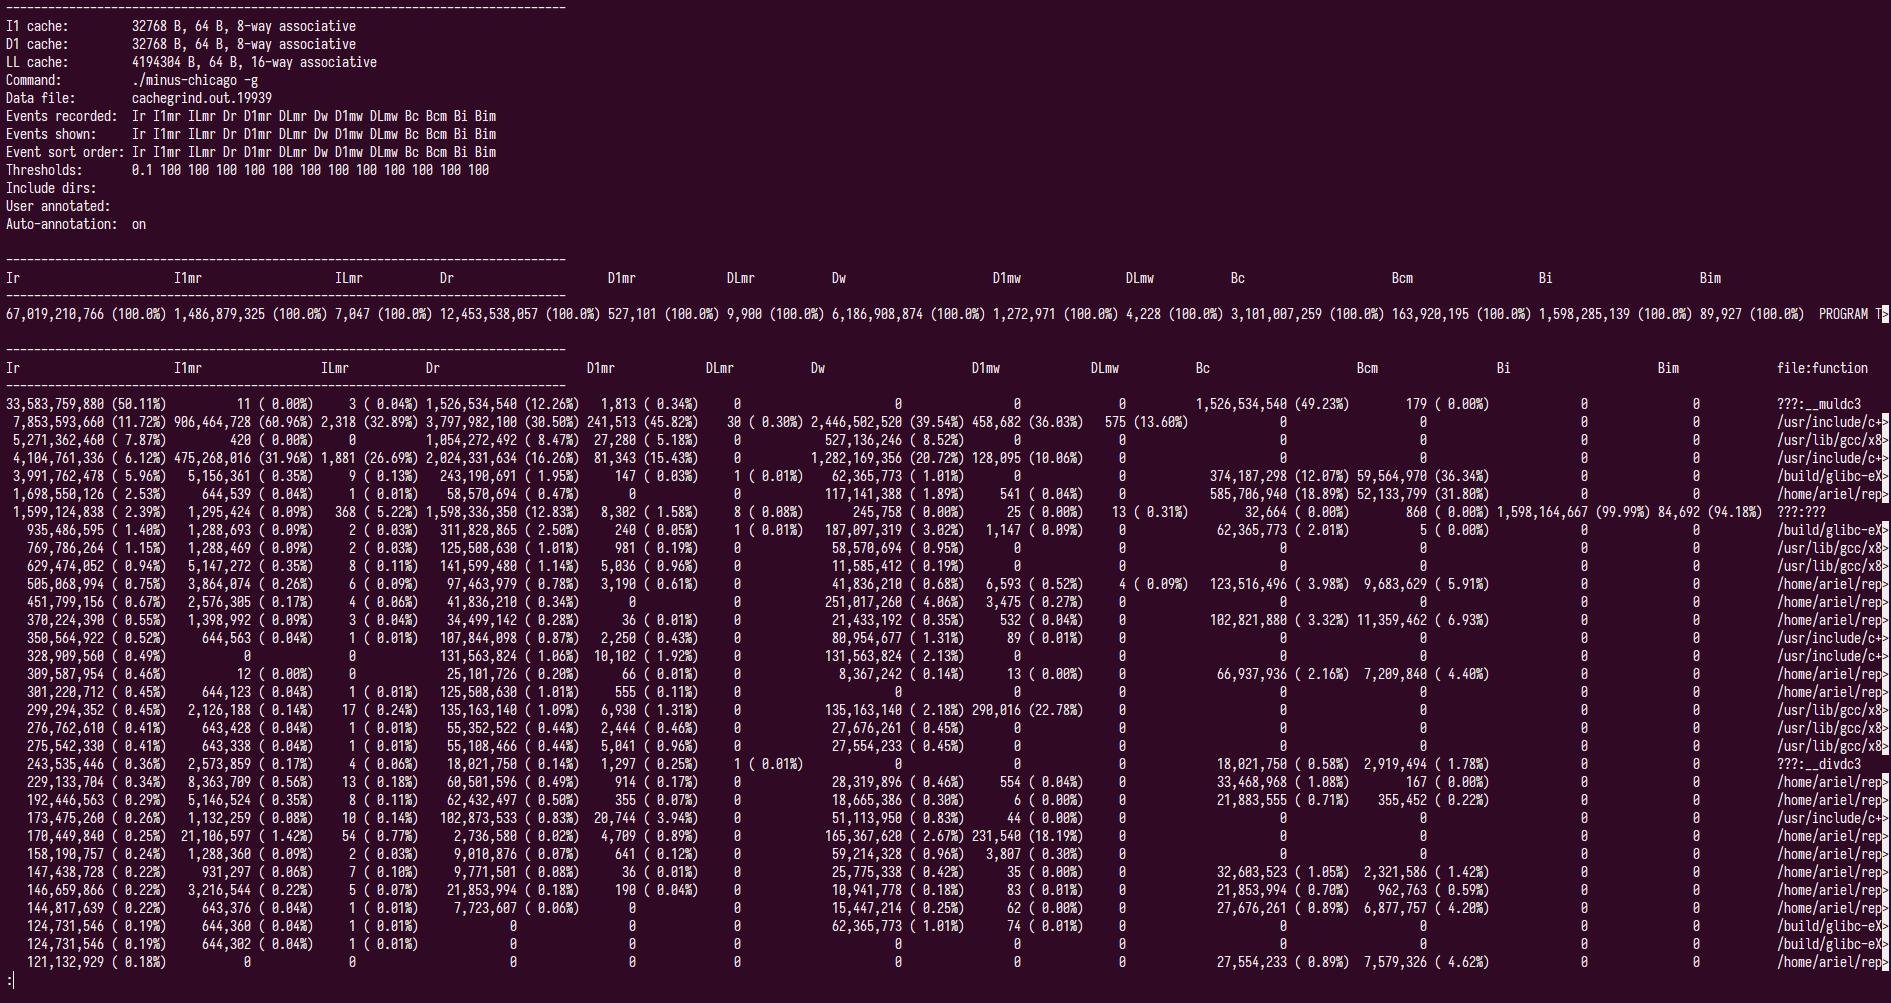
\includegraphics[width=\columnwidth]{figs/valgrind_cg_annotate0}
    \caption{Valgrind Cg\_annotate (Cachegrind\_annotate) 0}
\end{figure}
\begin{figure}[H]
    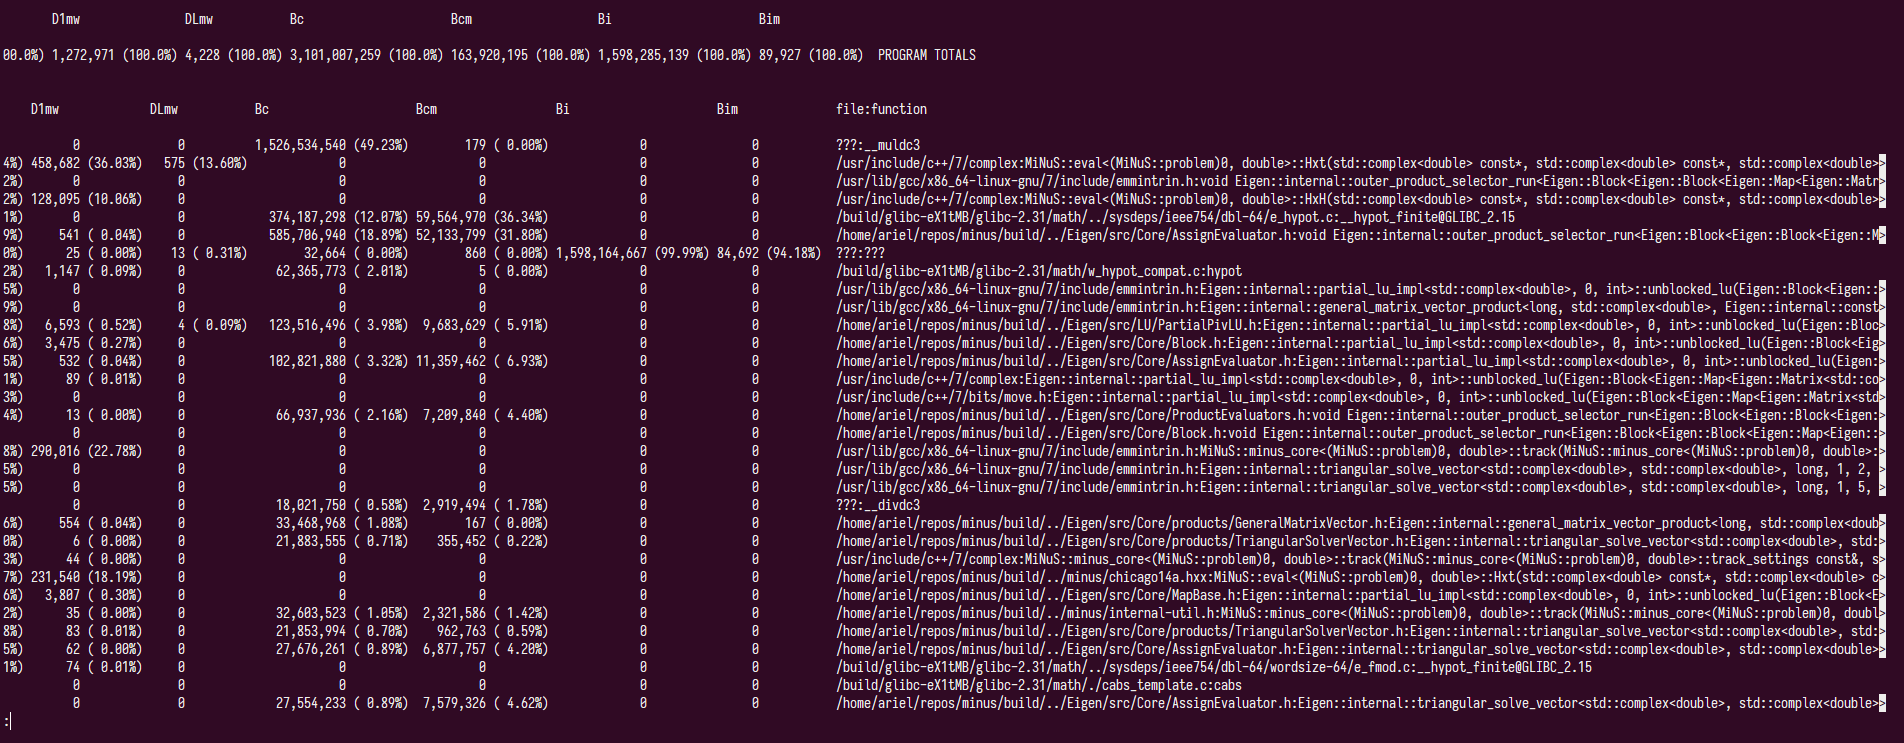
\includegraphics[width=\columnwidth]{figs/valgrind_cg_annotate1}
    \caption{Valgrind Cg\_annotate (Cachegrind\_annotate) 1}
\end{figure}

Using Callgrind in conjunction with the graphical tool QCachegrind, we can
see the function callers and callees, and what percentage of the total runtime
each one took. From this analysis, we can find that the most used function is
the GCC's library built-in complex multiplication routine, followed by the Eigen
library internal functions.

\begin{figure}[H]
    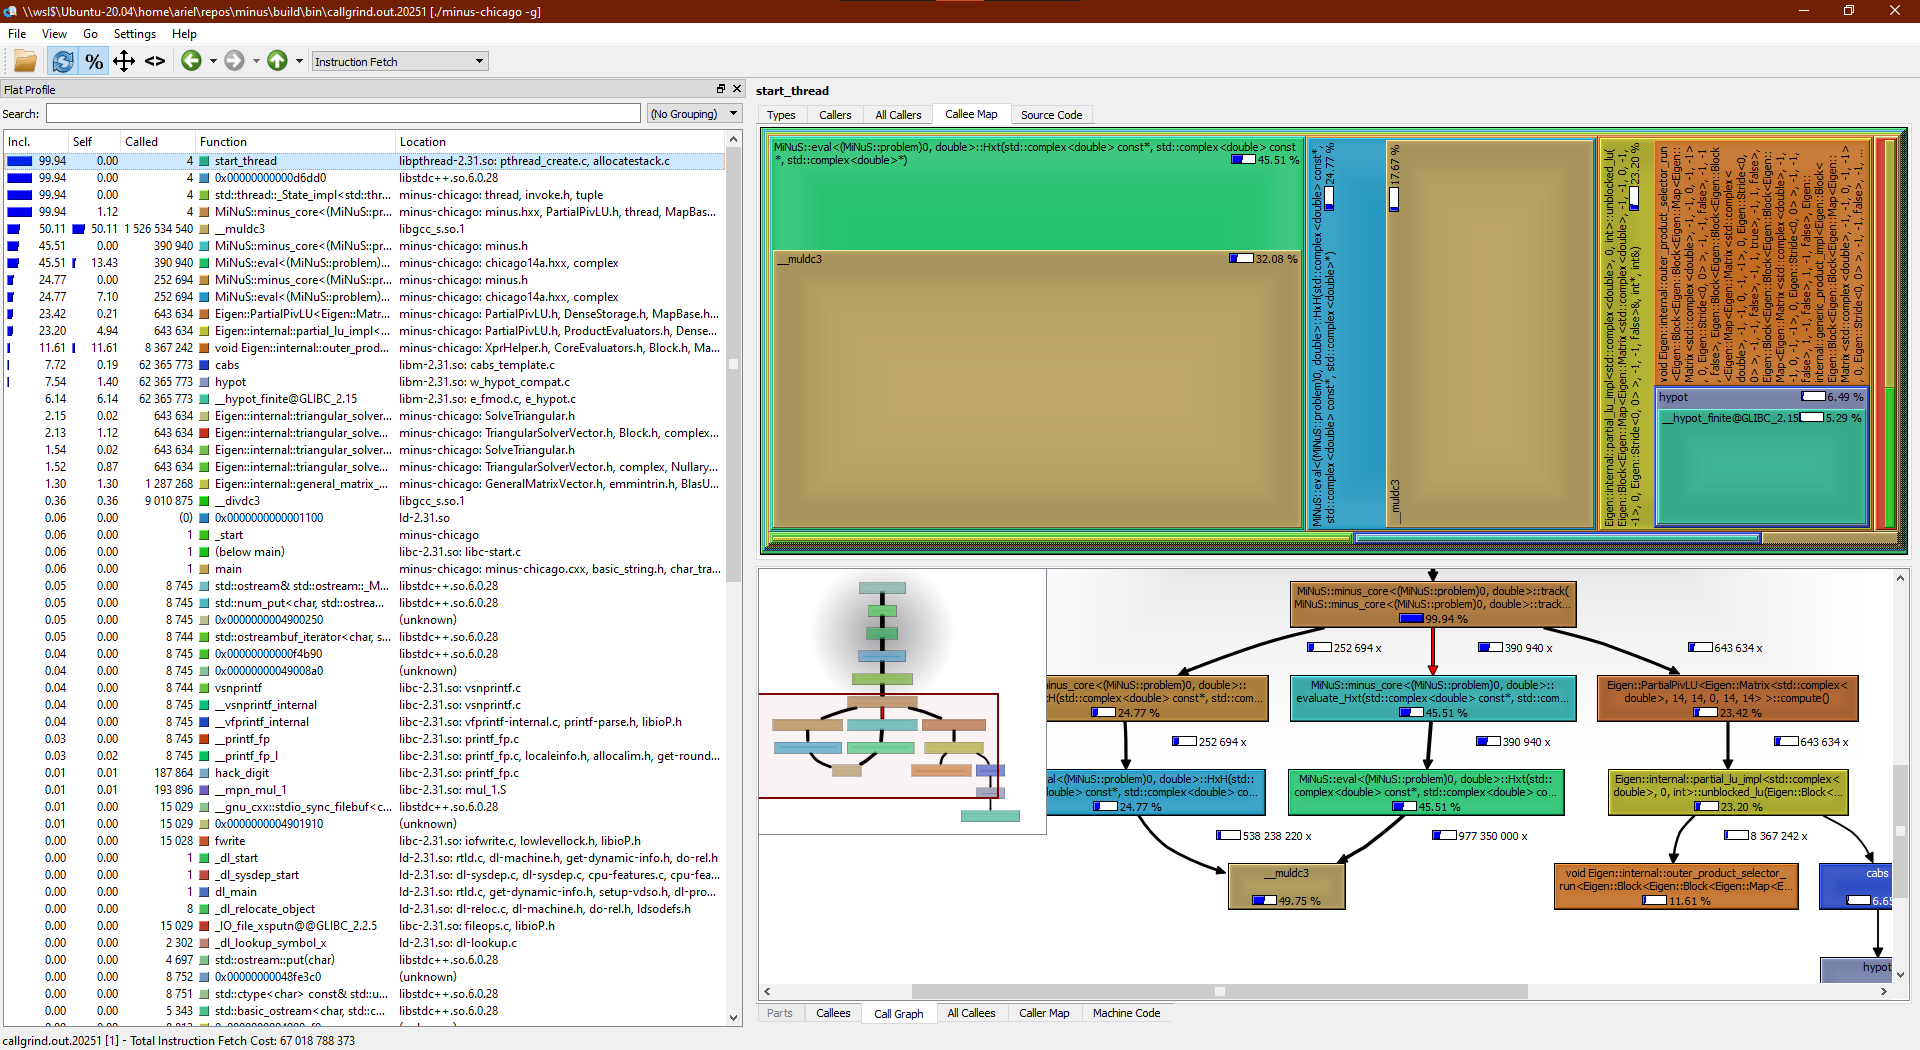
\includegraphics[width=\columnwidth]{figs/valgrind_qcachegrind_callgrind}
    \caption{Valgrind QCachegrind with Callgrind's output}
\end{figure}


\subsection{Graphical Analysis}

By tapping into the value of an element of each array we can try to detect
patterns which can be used to speedup certain calculations. For each iteration
of the main loop, we get a new value which is saved onto a text file. The lines
of this text file were loaded as an array of points in the online graphing tool
Desmos for graphical analysis.

Hxt[0]:
\begin{figure}[H]
    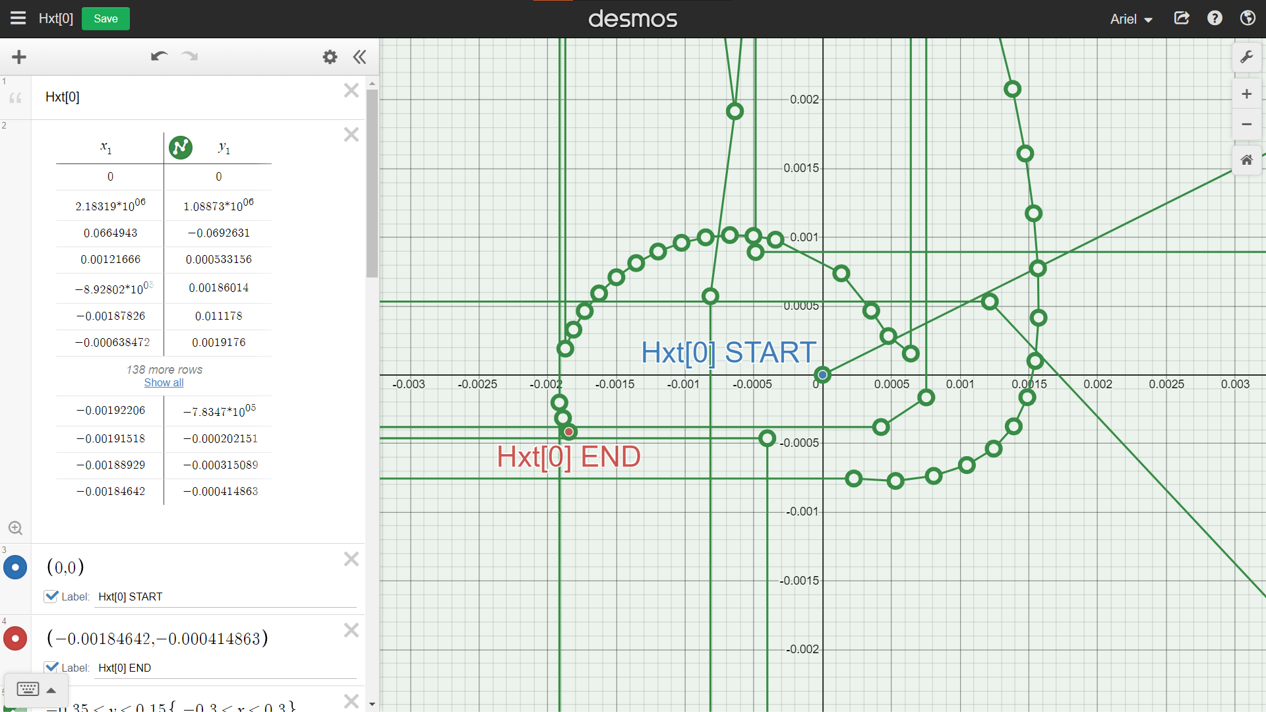
\includegraphics[width=\columnwidth]{figs/Hxt[0]_0}
    \caption{Hxt[0] 0}
\end{figure}
\begin{figure}[H]
    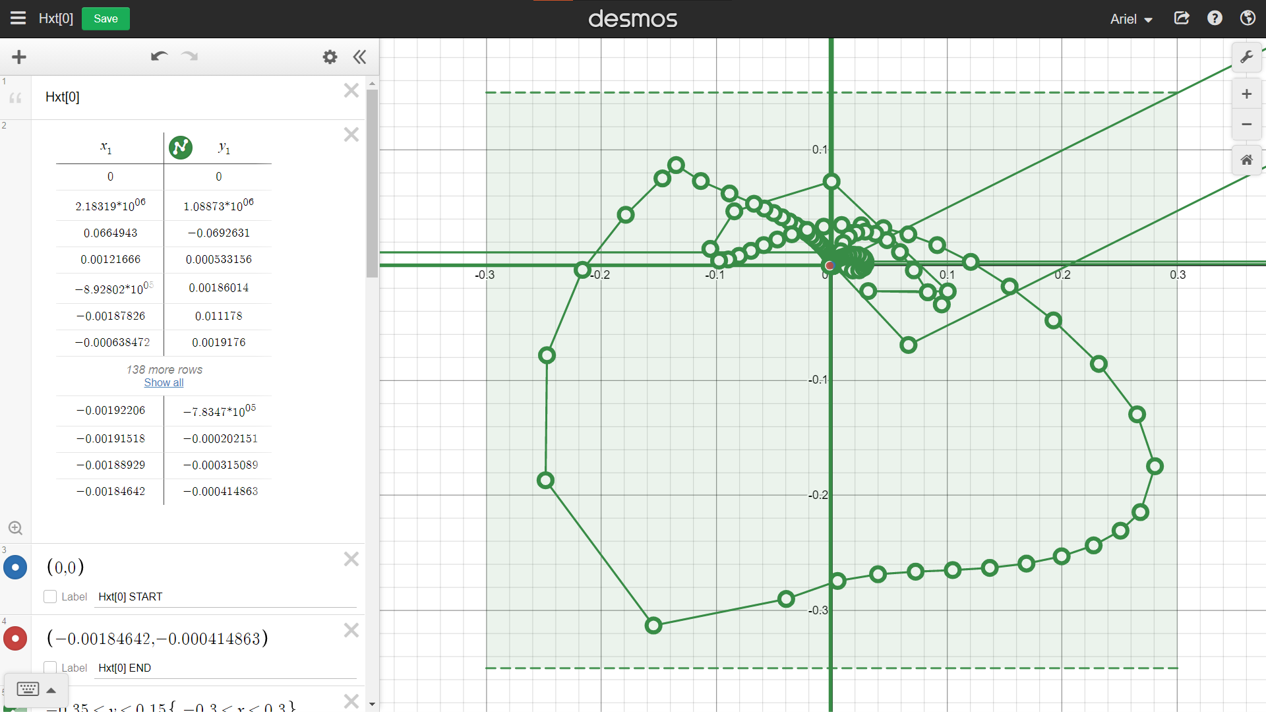
\includegraphics[width=\columnwidth]{figs/Hxt[0]_1}
    \caption{Hxt[0] 1}
\end{figure}
\begin{figure}[H]
    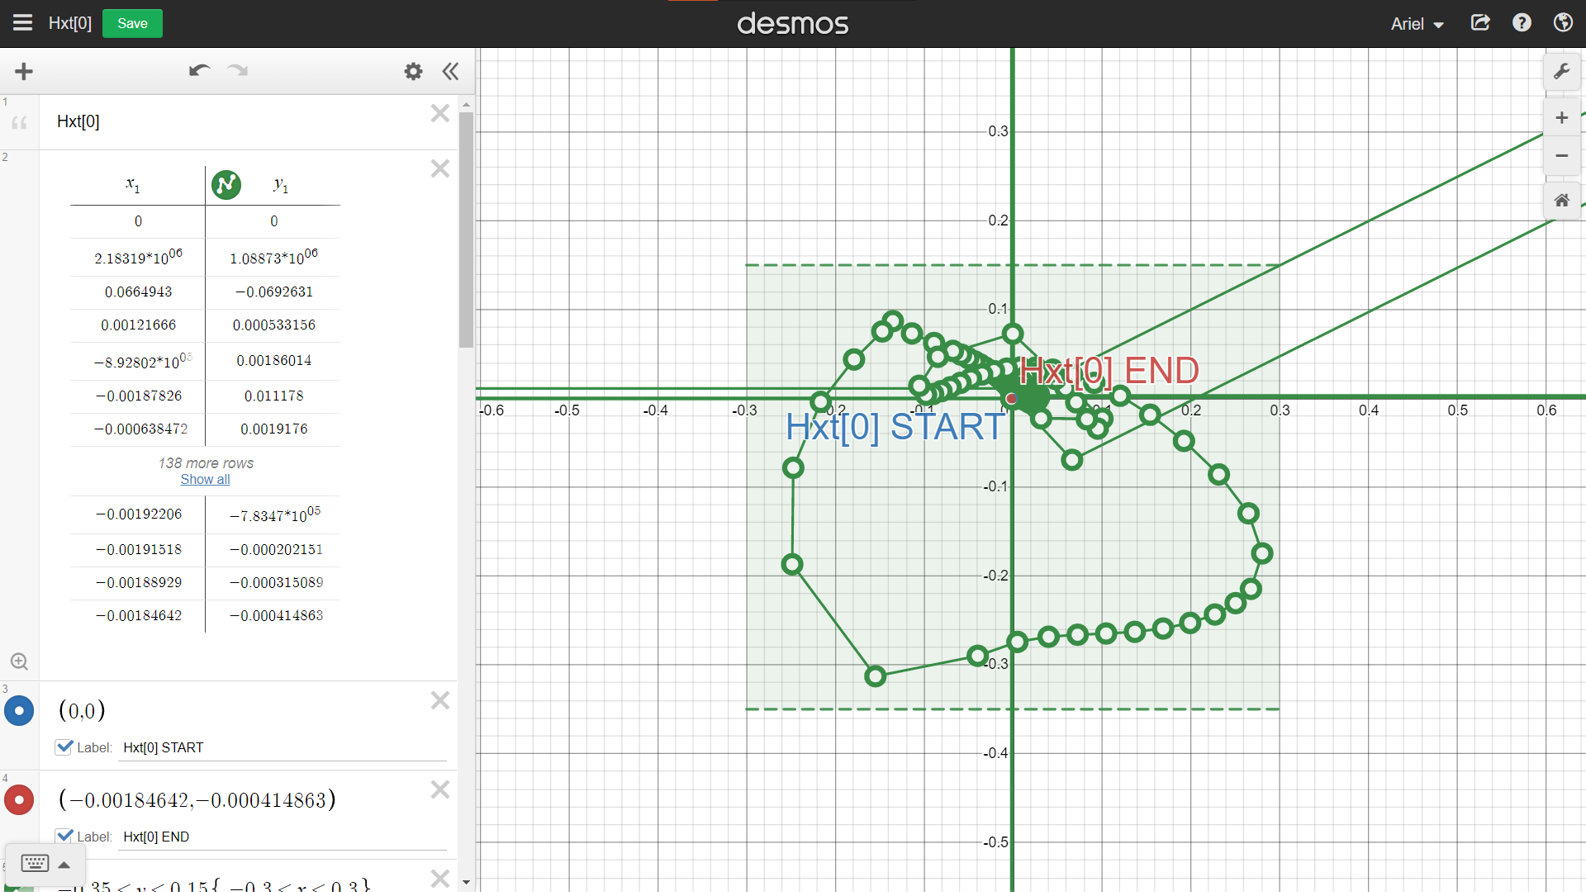
\includegraphics[width=\columnwidth]{figs/Hxt[0]_2}
    \caption{Hxt[0] 2}
\end{figure}
\begin{figure}[H]
    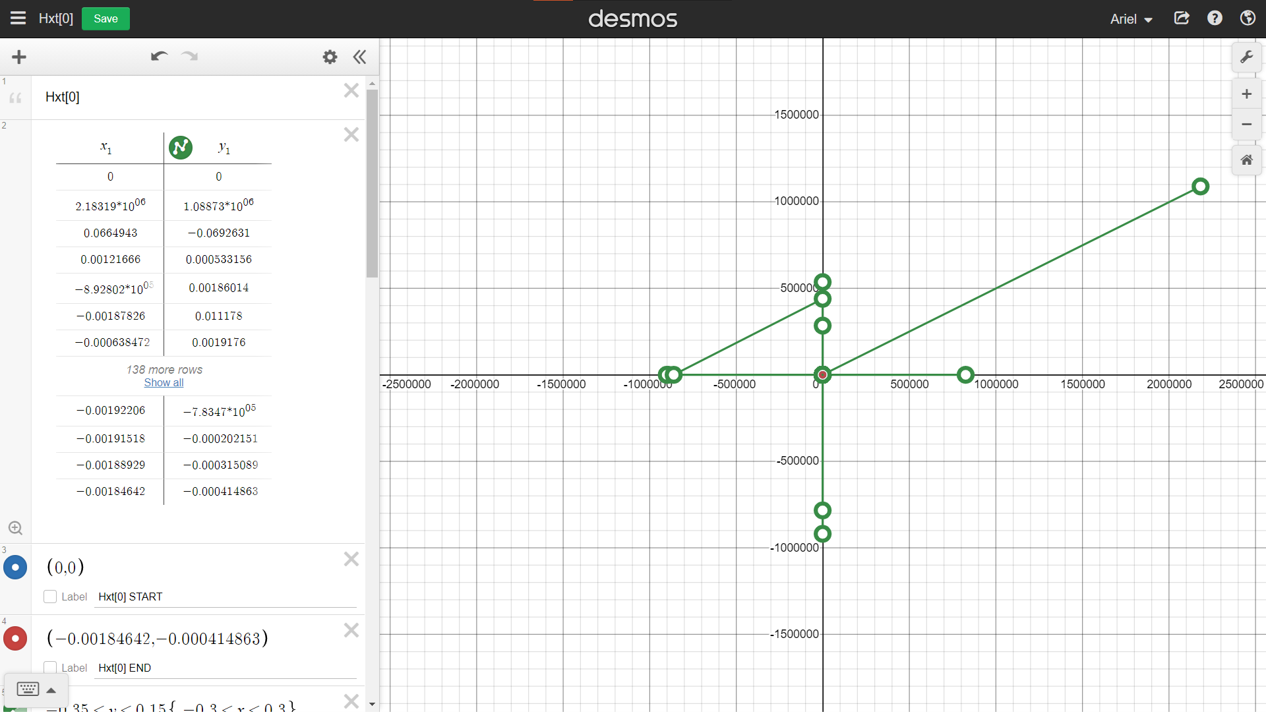
\includegraphics[width=\columnwidth]{figs/Hxt[0]_3}
    \caption{Hxt[0] 3}
\end{figure}
\begin{figure}[H]
    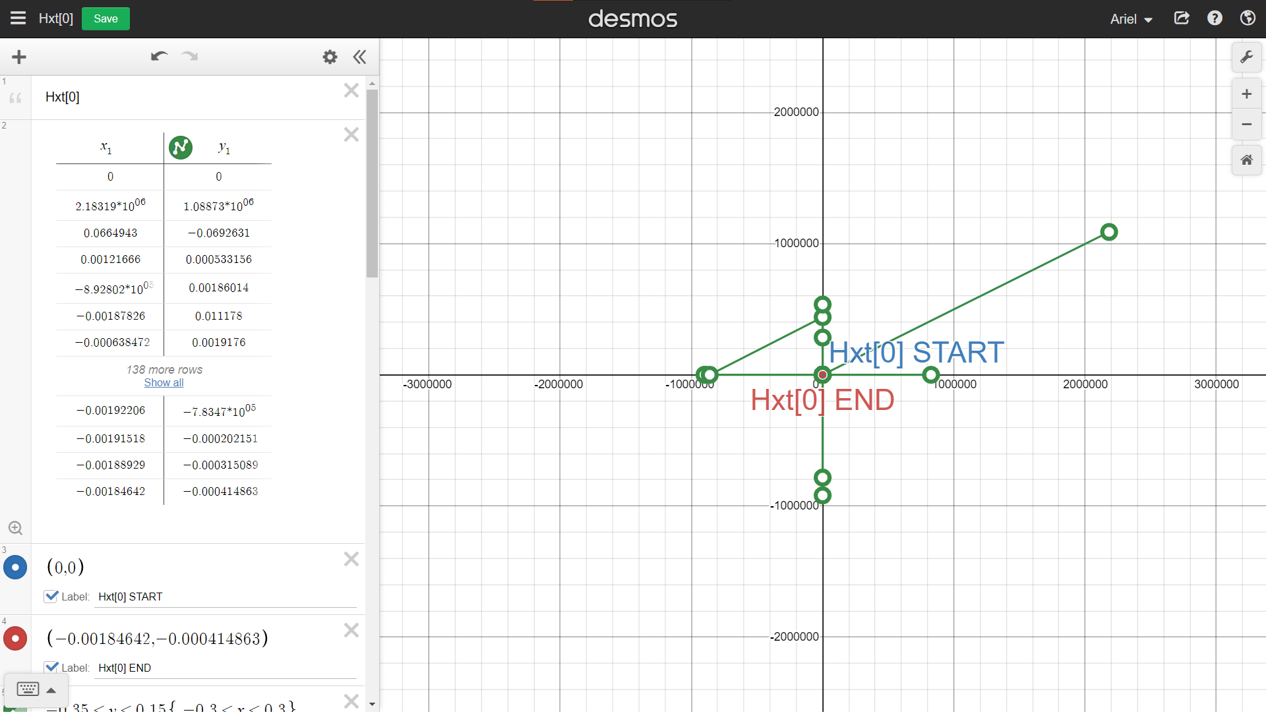
\includegraphics[width=\columnwidth]{figs/Hxt[0]_4}
    \caption{Hxt[0] 4}
\end{figure}

dxdi[0]:
\begin{figure}[H]
    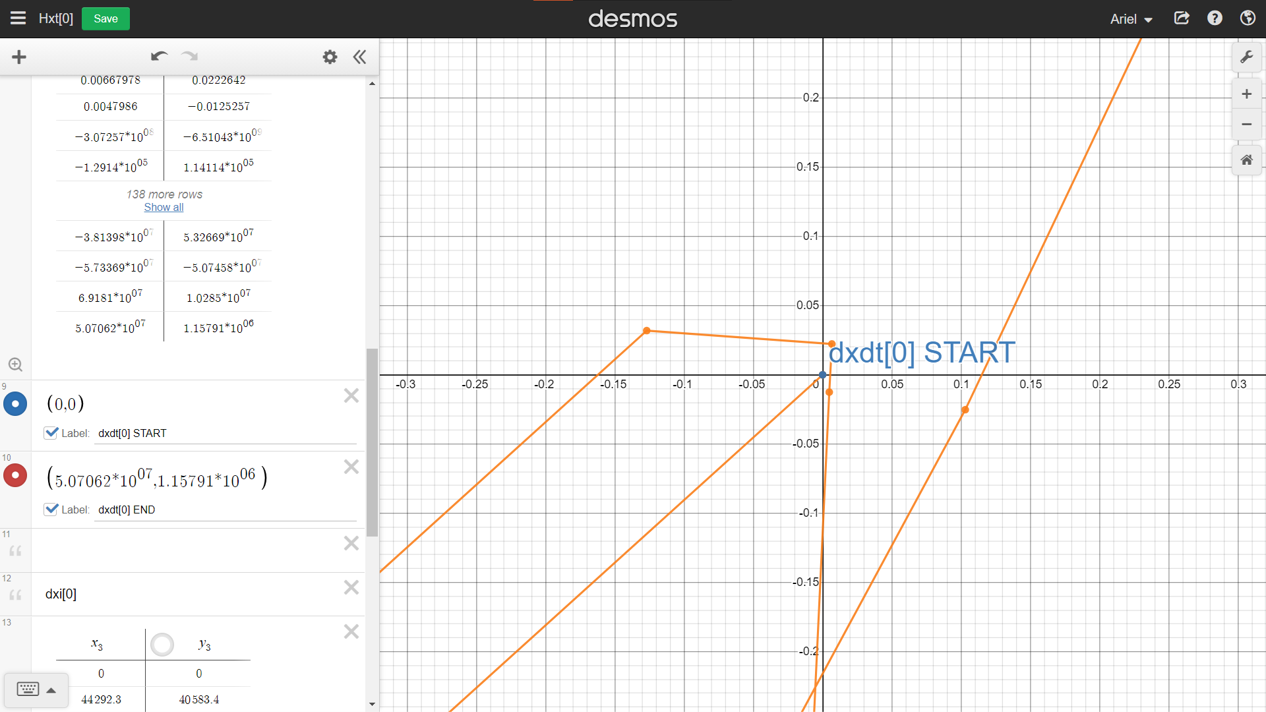
\includegraphics[width=\columnwidth]{figs/dxdi[0]_0}
    \caption{dxdi[0] 0}
\end{figure}
\begin{figure}[H]
    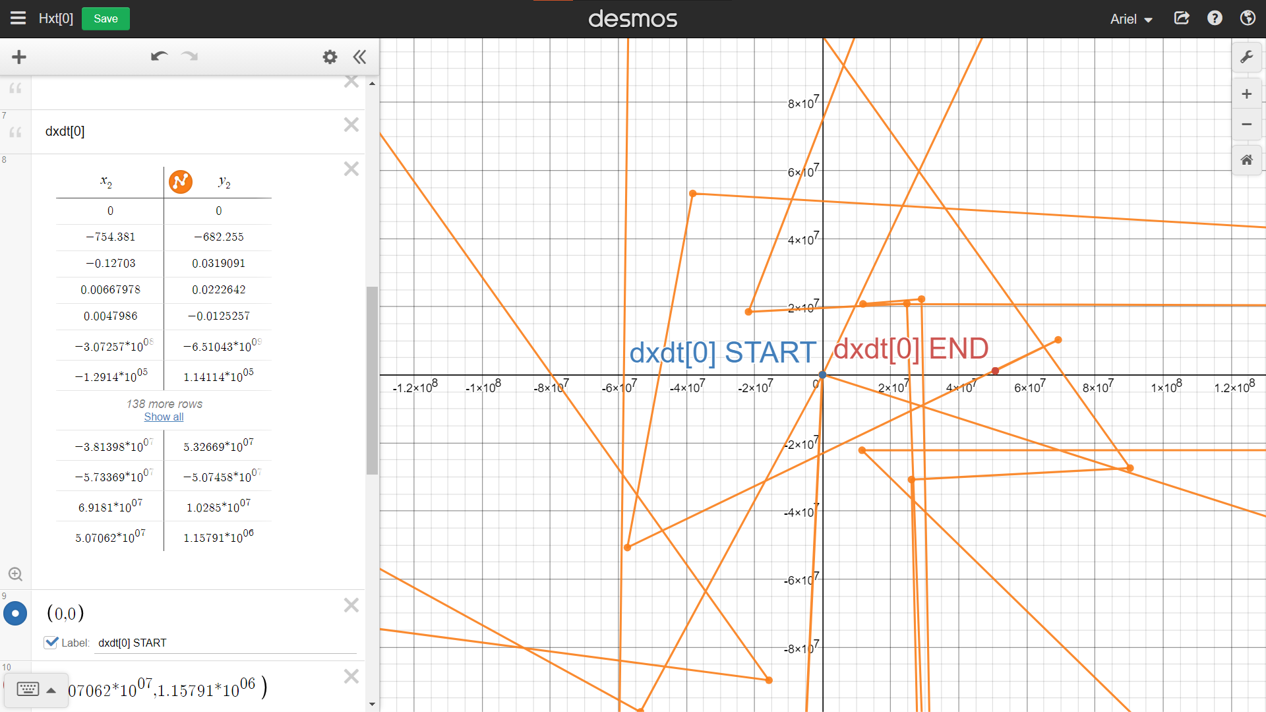
\includegraphics[width=\columnwidth]{figs/dxdi[0]_1}
    \caption{dxdi[0] 1}
\end{figure}
\begin{figure}[H]
    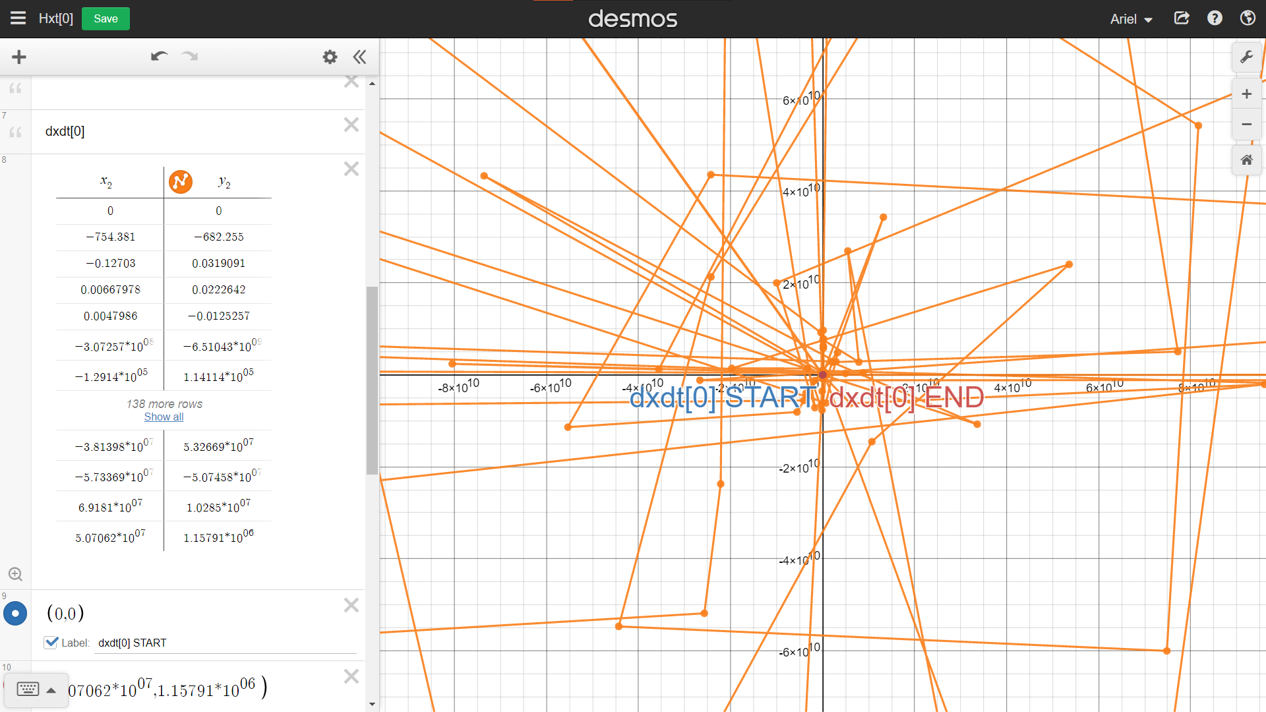
\includegraphics[width=\columnwidth]{figs/dxdi[0]_2}
    \caption{dxdi[0] 2}
\end{figure}
\begin{figure}[H]
    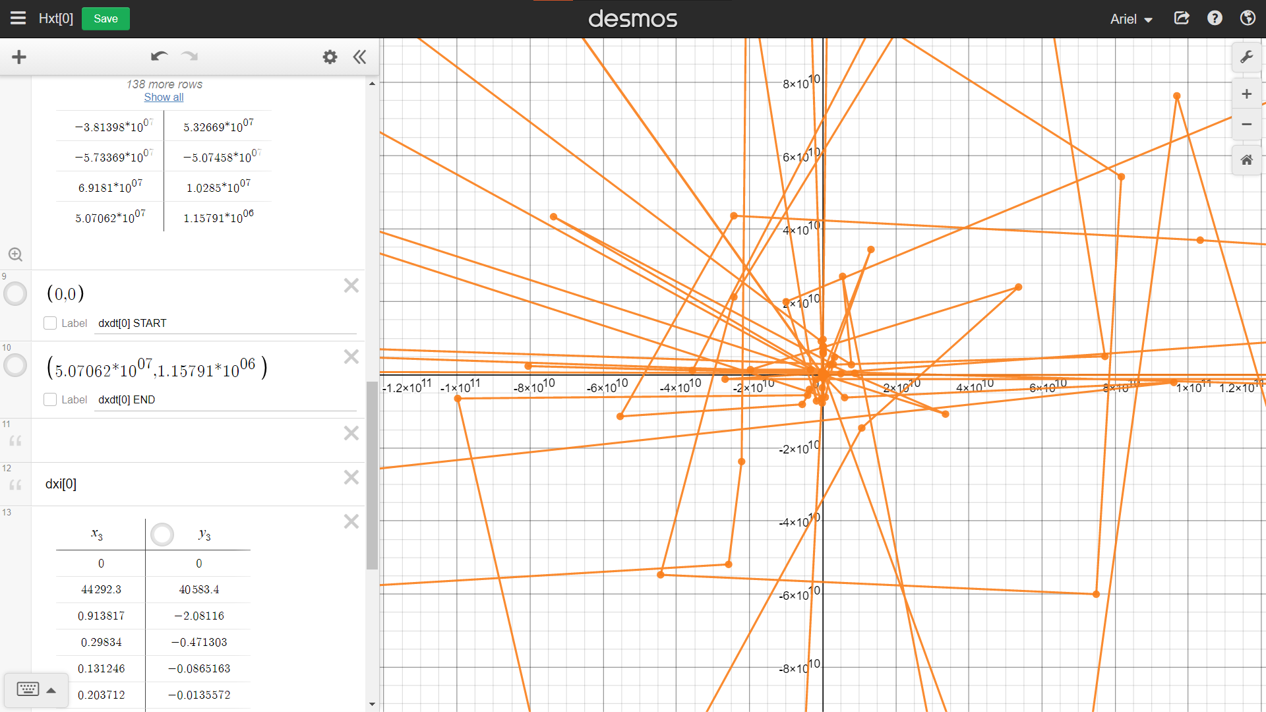
\includegraphics[width=\columnwidth]{figs/dxdi[0]_3}
    \caption{dxdi[0] 3}
\end{figure}
\begin{figure}[H]
    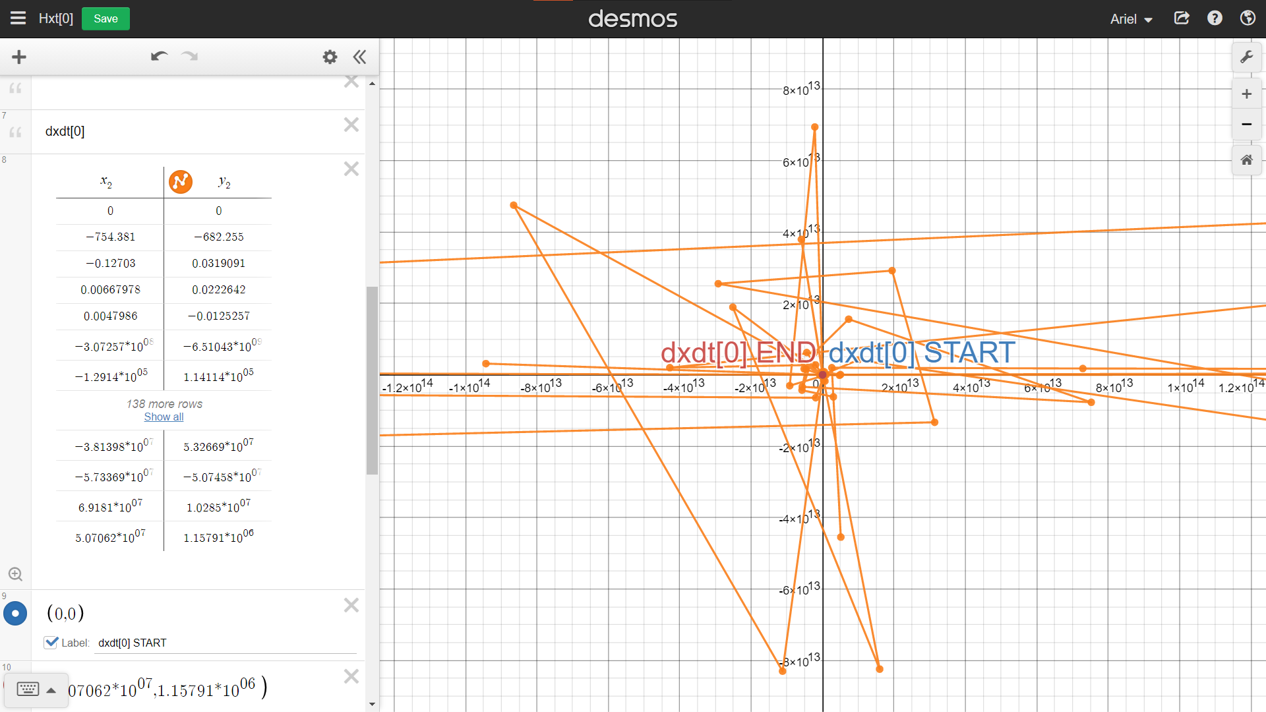
\includegraphics[width=\columnwidth]{figs/dxdi[0]_4}
    \caption{dxdi[0] 4}
\end{figure}
\begin{figure}[H]
    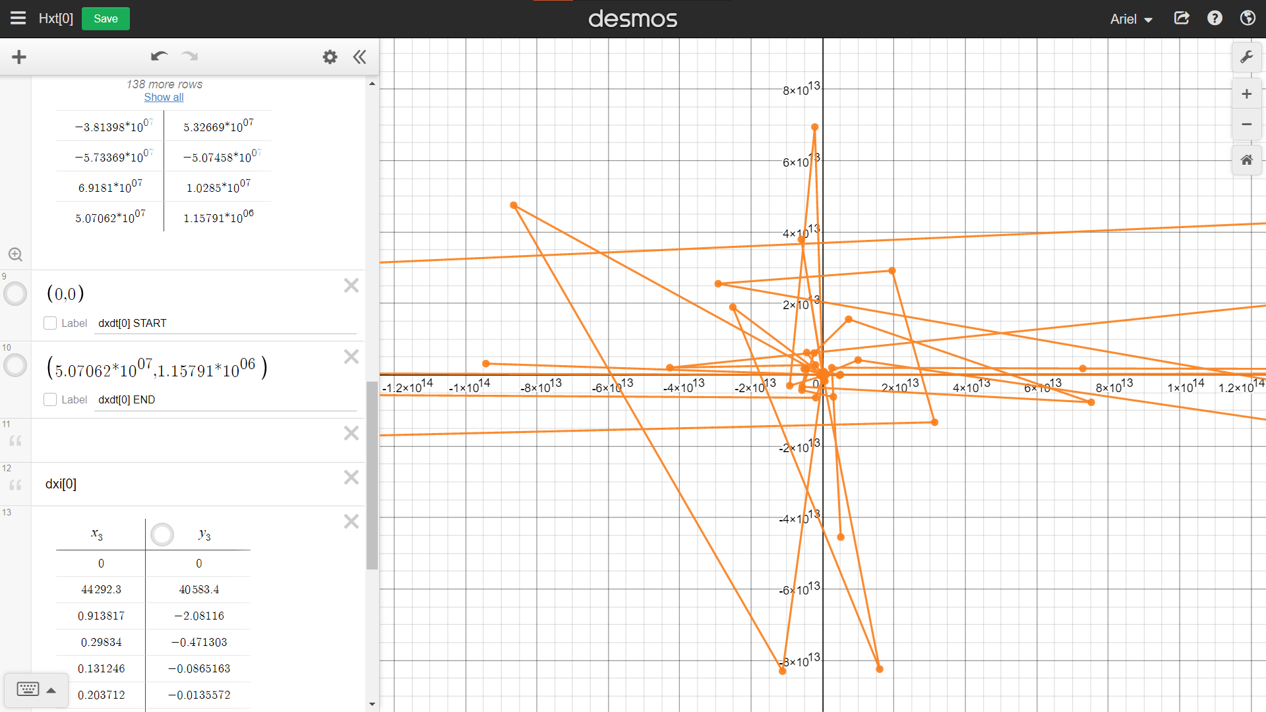
\includegraphics[width=\columnwidth]{figs/dxdi[0]_5}
    \caption{dxdi[0] 5}
\end{figure}
\begin{figure}[H]
    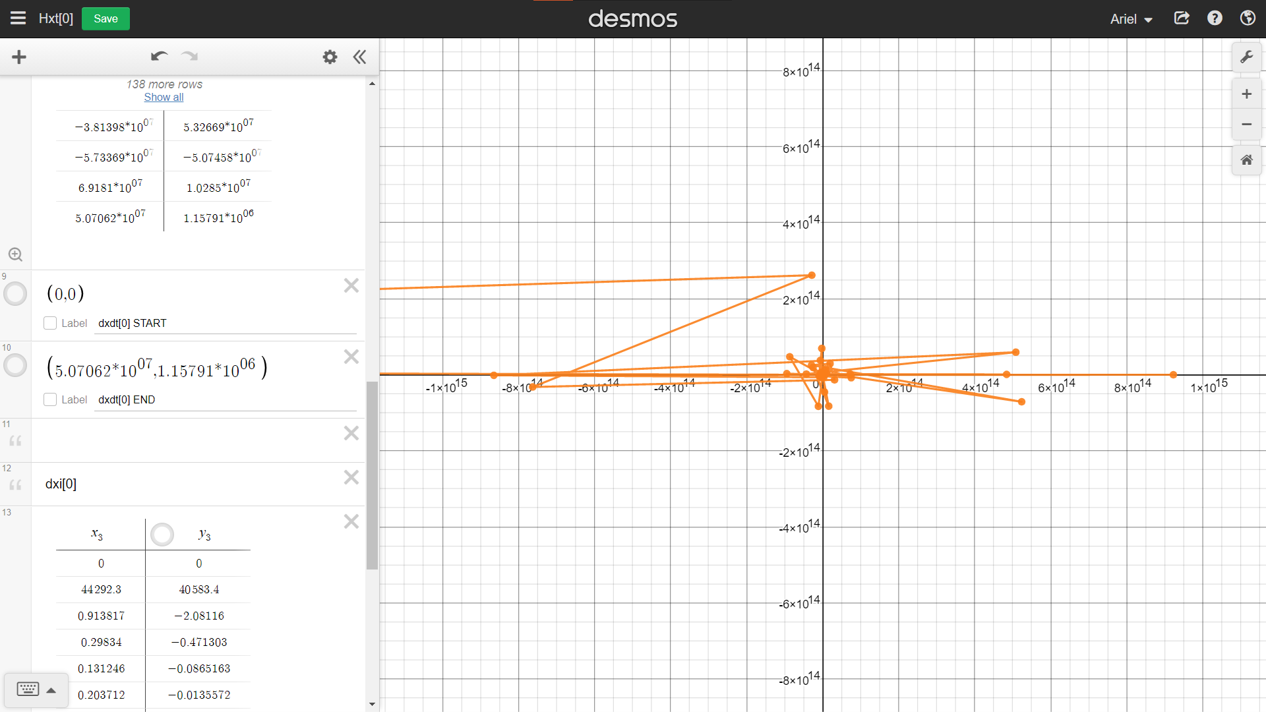
\includegraphics[width=\columnwidth]{figs/dxdi[0]_6}
    \caption{dxdi[0] 6}
\end{figure}
\begin{figure}[H]
    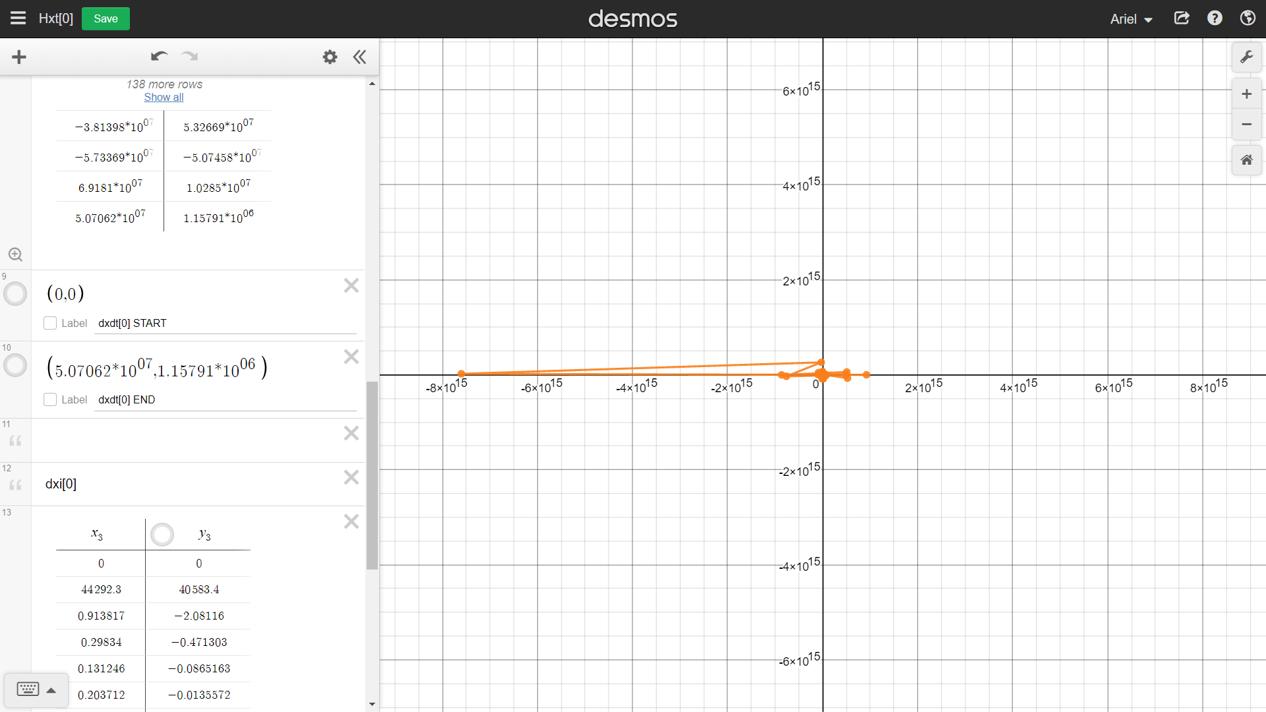
\includegraphics[width=\columnwidth]{figs/dxdi[0]_7}
    \caption{dxdi[0] 7}
\end{figure}

dxi[0]:
\begin{figure}[H]
    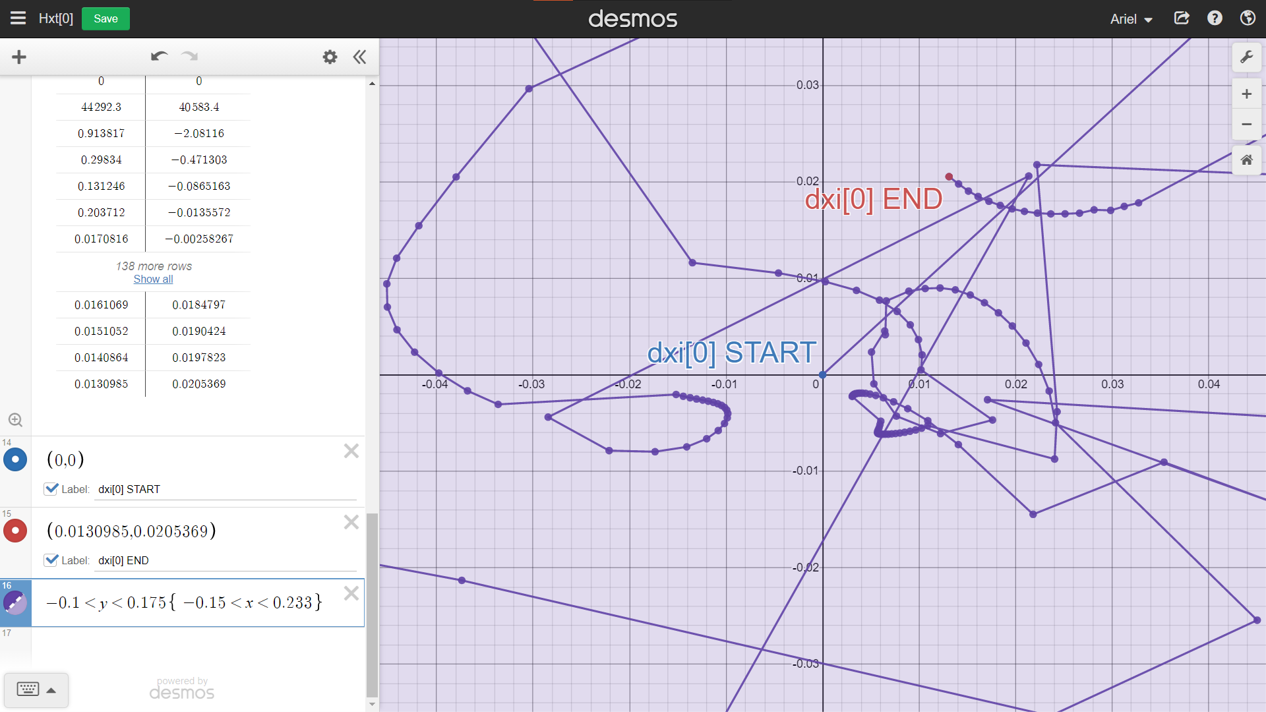
\includegraphics[width=\columnwidth]{figs/dxi[0]_0}
    \caption{dxi[0] 0}
\end{figure}
\begin{figure}[H]
    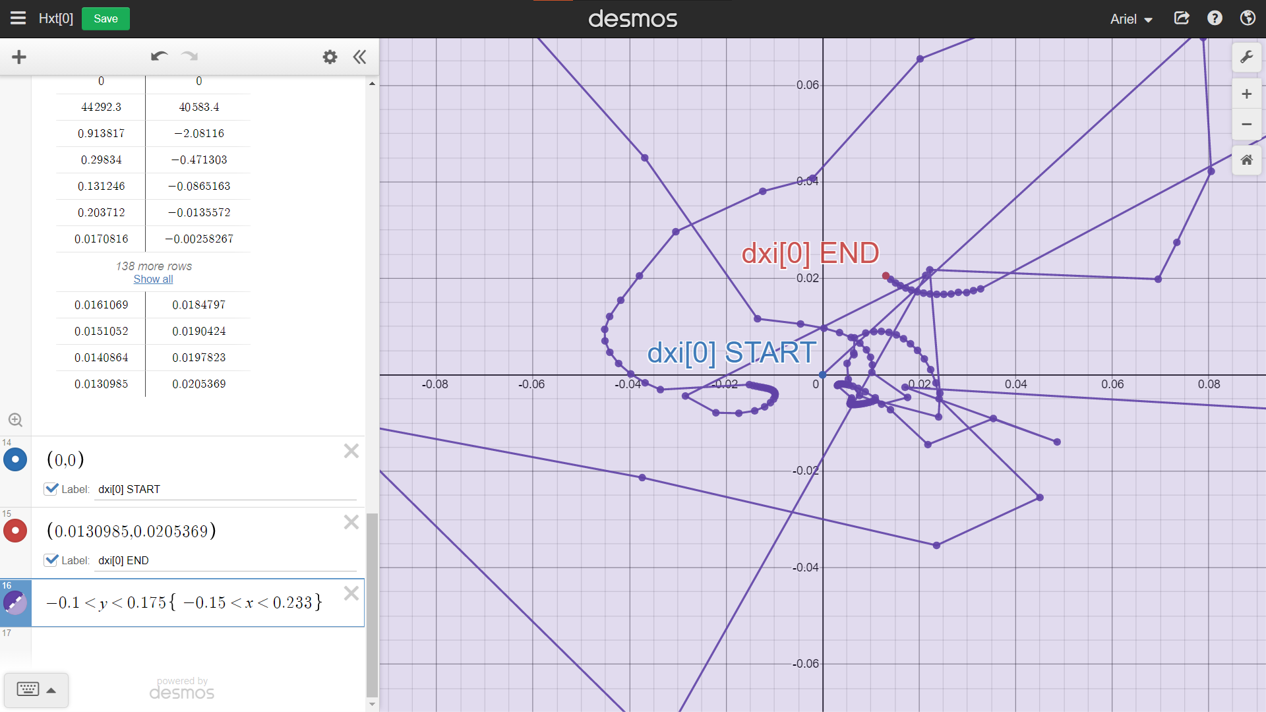
\includegraphics[width=\columnwidth]{figs/dxi[0]_1}
    \caption{dxi[0] 1}
\end{figure}
\begin{figure}[H]
    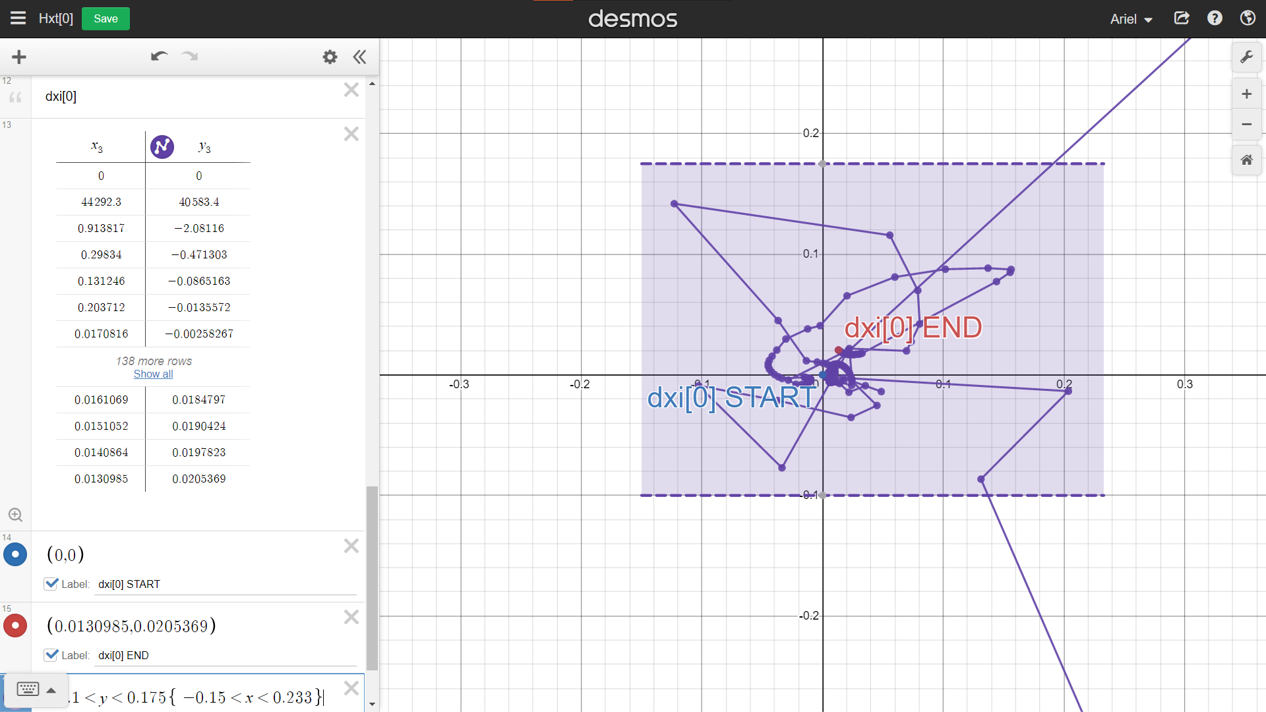
\includegraphics[width=\columnwidth]{figs/dxi[0]_2}
    \caption{dxi[0] 2}
\end{figure}
\begin{figure}[H]
    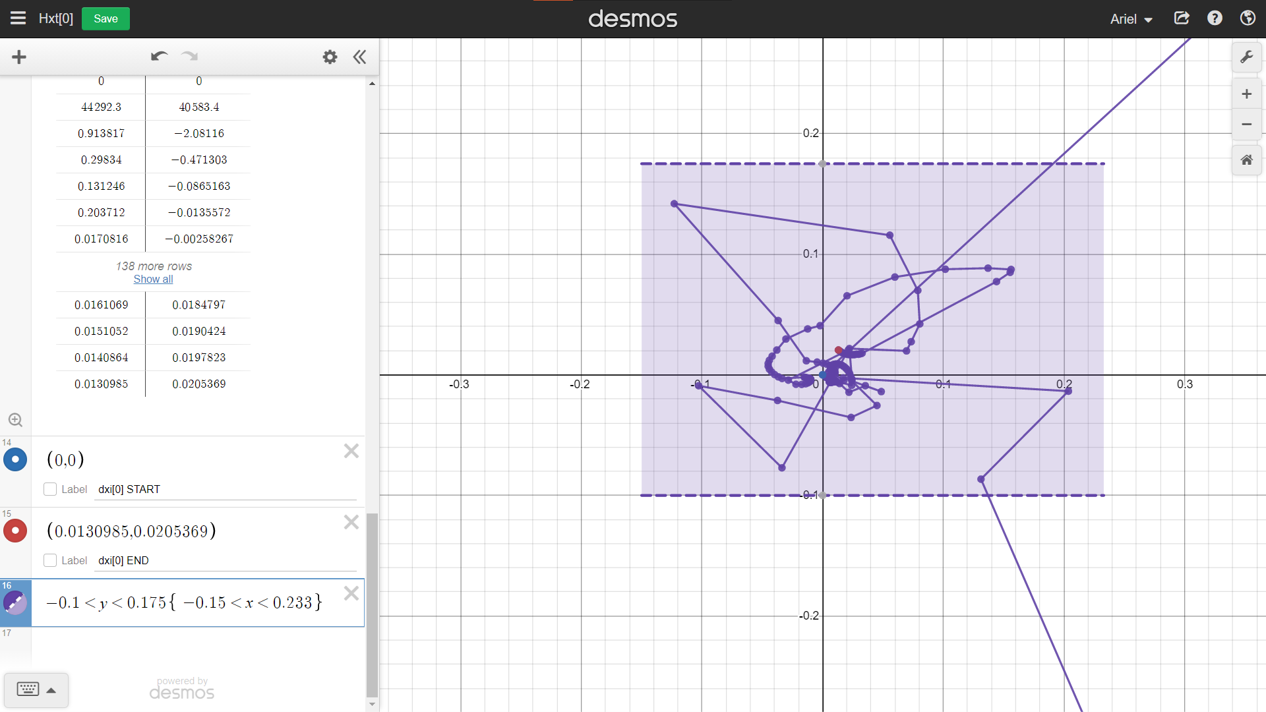
\includegraphics[width=\columnwidth]{figs/dxi[0]_3}
    \caption{dxi[0] 3}
\end{figure}
\begin{figure}[H]
    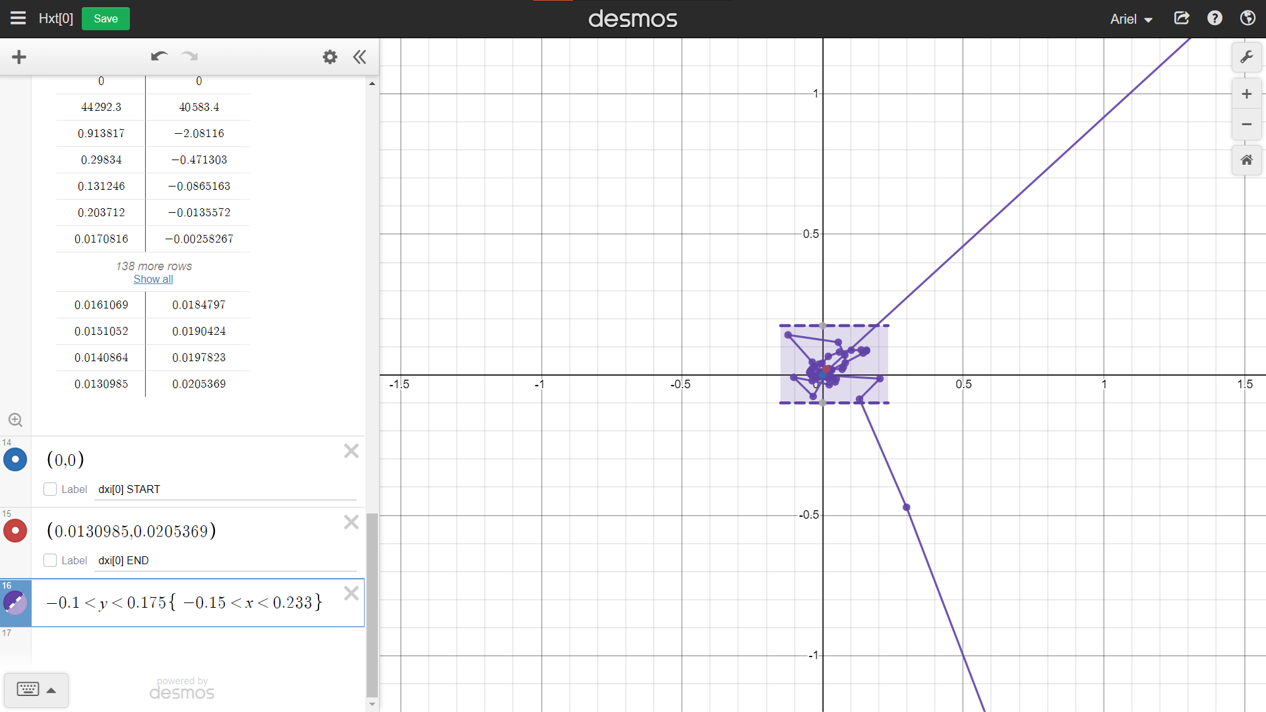
\includegraphics[width=\columnwidth]{figs/dxi[0]_4}
    \caption{dxi[0] 4}
\end{figure}
\begin{figure}[H]
    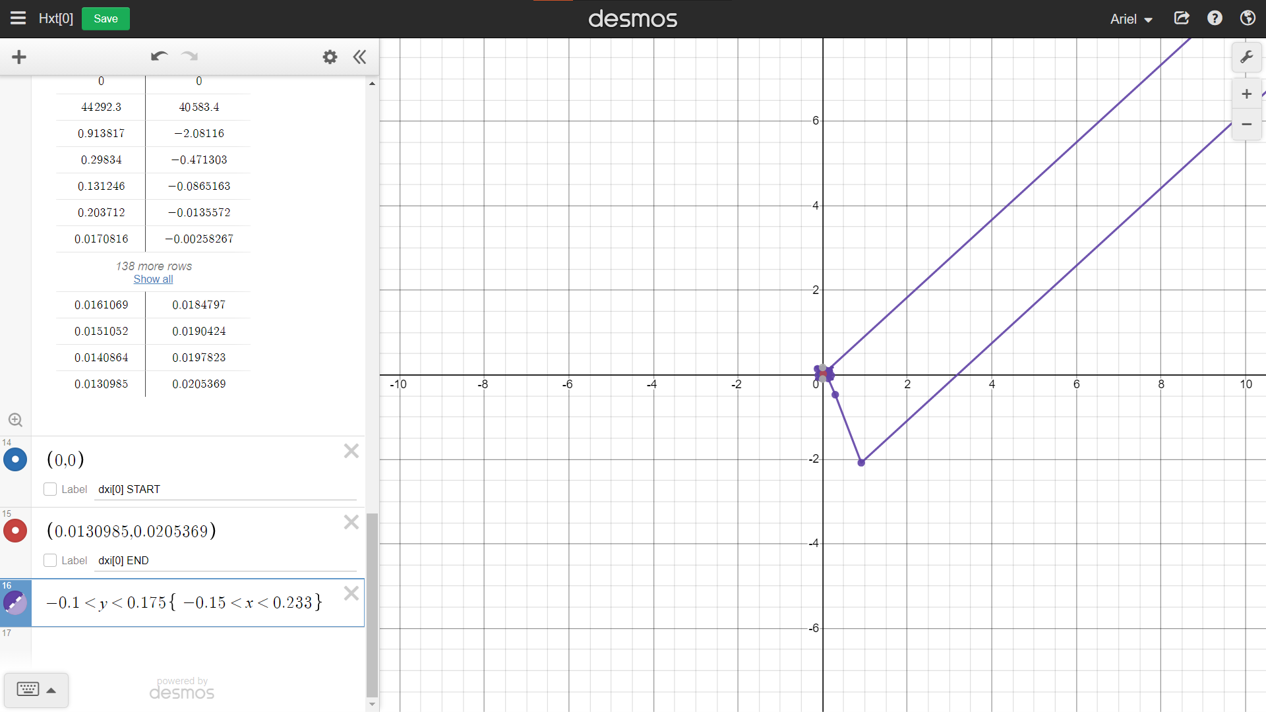
\includegraphics[width=\columnwidth]{figs/dxi[0]_5}
    \caption{dxi[0] 5}
\end{figure}
\begin{figure}[H]
    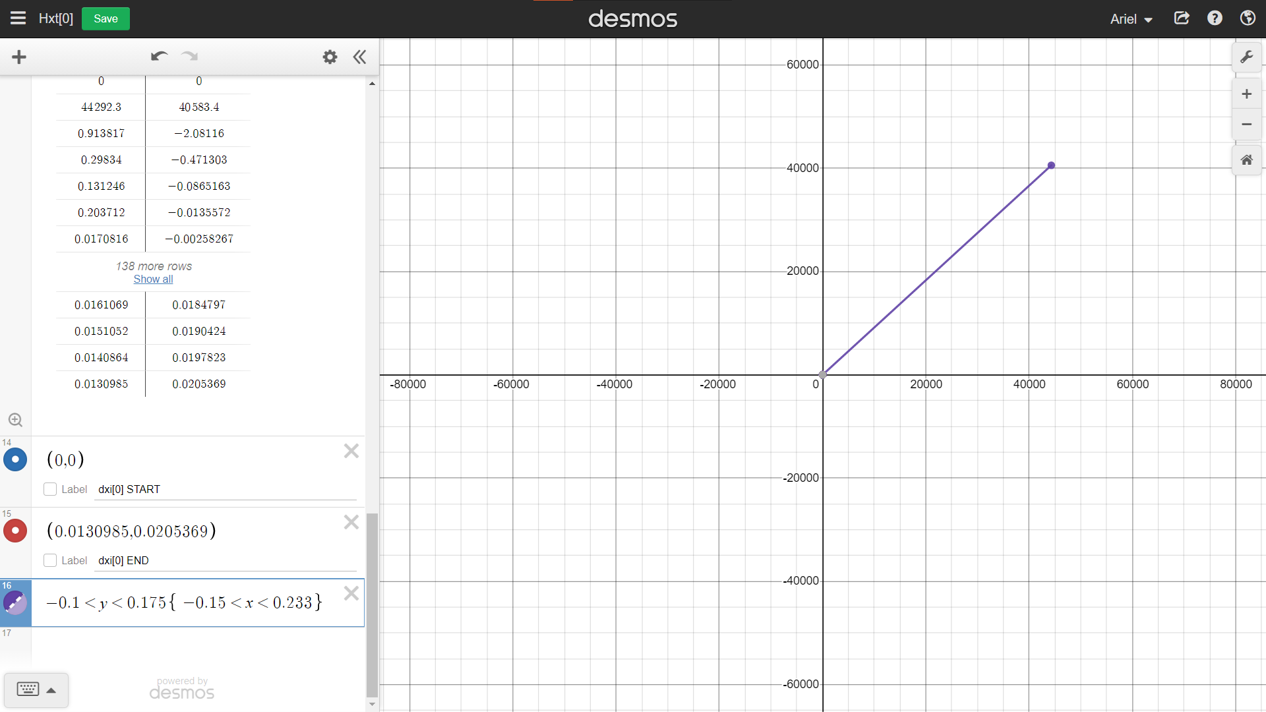
\includegraphics[width=\columnwidth]{figs/dxi[0]_6}
    \caption{dxi[0] 6}
\end{figure}


\subsection{Benchmarking Changes}
By allocating a single memory block and manually assigning pointers to specific
positions, we can eliminate the memory gap created by the compiler. Furthermore,
by using the special keyword \verb|__restrict__|, it's possible for the compiler
to optimize the code more thoroughly, as we promise it we won't cause any
pointer aliasing.

We benchmarked the program before and after the changes, and noticed a small
speedup. This may be due to fewer cache misses, as the most frequently accessed
memory segment is smaller in size.

Benchmark results:

Benchmark 20 tries before change
\footnotesize\begin{verbatim}
        Running test 1/20: 1.78s
        Running test 2/20: 1.47s
        Running test 3/20: 1.81s
        Running test 4/20: 1.52s
        Running test 5/20: 1.75s
        Running test 6/20: 1.51s
        Running test 7/20: 1.48s
        Running test 8/20: 1.42s
        Running test 9/20: 1.40s
        Running test 10/20: 1.50s
        Running test 11/20: 1.54s
        Running test 12/20: 1.44s
        Running test 13/20: 1.46s
        Running test 14/20: 1.45s
        Running test 15/20: 1.41s
        Running test 16/20: 1.48s
        Running test 17/20: 1.70s
        Running test 18/20: 1.65s
        Running test 19/20: 1.72s
        Running test 20/20: 1.81s
        AVERAGE TIME (20 RUNS): 1.56s
\end{verbatim}
\normalsize

Benchmark 20 tries after change:
\footnotesize\begin{verbatim}
    Running test 1/20: 1.54s
    Running test 2/20: 1.40s
    Running test 3/20: 1.42s
    Running test 4/20: 1.39s
    Running test 5/20: 1.40s
    Running test 6/20: 1.40s
    Running test 7/20: 1.45s
    Running test 8/20: 1.37s
    Running test 9/20: 1.38s
    Running test 10/20: 1.42s
    Running test 11/20: 1.38s
    Running test 12/20: 1.41s
    Running test 13/20: 1.37s
    Running test 14/20: 1.82s
    Running test 15/20: 1.47s
    Running test 16/20: 1.85s
    Running test 17/20: 1.71s
    Running test 18/20: 1.42s
    Running test 19/20: 1.54s
    Running test 20/20: 1.65s
    AVERAGE TIME (20 RUNS): 1.49s
\end{verbatim}
\normalsize

Benchmark 20 tries after change with \verb|__restrict__|
\footnotesize\begin{verbatim}
    Running test 1/20: 1.53s
    Running test 2/20: 1.44s
    Running test 3/20: 1.41s
    Running test 4/20: 1.40s
    Running test 5/20: 1.47s
    Running test 6/20: 1.41s
    Running test 7/20: 1.41s
    Running test 8/20: 1.42s
    Running test 9/20: 1.42s
    Running test 10/20: 1.40s
    Running test 11/20: 1.38s
    Running test 12/20: 1.44s
    Running test 13/20: 1.39s
    Running test 14/20: 1.41s
    Running test 15/20: 1.98s
    Running test 16/20: 2.01s
    Running test 17/20: 1.43s
    Running test 18/20: 1.47s
    Running test 19/20: 1.81s
    Running test 20/20: 1.57s
    AVERAGE TIME (20 RUNS): 1.51s
\end{verbatim}
\normalsize

Benchmark 5 rounds 10 tries before change
\footnotesize\begin{verbatim}
    Round 1/5
        Running test 1/10: 1440ms
        Running test 2/10: 1373ms
        Running test 3/10: 1374ms
        Running test 4/10: 1451ms
        Running test 5/10: 1409ms
        Running test 6/10: 1400ms
        Running test 7/10: 1380ms
        Running test 8/10: 1401ms
        Running test 9/10: 1397ms
        Running test 10/10: 1416ms
        AVERAGE TIME (FIRST 5 RUNS): 1409.400ms
        AVERAGE TIME (10 RUNS): 1404.100ms
    Round finished. Sleeping for 10 seconds...
    Round 2/5
        Running test 1/10: 1392ms
        Running test 2/10: 1385ms
        Running test 3/10: 1411ms
        Running test 4/10: 1375ms
        Running test 5/10: 1410ms
        Running test 6/10: 1401ms
        Running test 7/10: 1387ms
        Running test 8/10: 1528ms
        Running test 9/10: 1714ms
        Running test 10/10: 1596ms
        AVERAGE TIME (FIRST 5 RUNS): 1394.600ms
        AVERAGE TIME (10 RUNS): 1459.900ms
    Round finished. Sleeping for 10 seconds...
    Round 3/5
        Running test 1/10: 1399ms
        Running test 2/10: 1376ms
        Running test 3/10: 1390ms
        Running test 4/10: 1397ms
        Running test 5/10: 1381ms
        Running test 6/10: 1405ms
        Running test 7/10: 1407ms
        Running test 8/10: 1550ms
        Running test 9/10: 1629ms
        Running test 10/10: 1656ms
        AVERAGE TIME (FIRST 5 RUNS): 1388.600ms
        AVERAGE TIME (10 RUNS): 1459.000ms
    Round finished. Sleeping for 10 seconds...
    Round 4/5
        Running test 1/10: 1402ms
        Running test 2/10: 1394ms
        Running test 3/10: 1398ms
        Running test 4/10: 1416ms
        Running test 5/10: 1421ms
        Running test 6/10: 1413ms
        Running test 7/10: 1435ms
        Running test 8/10: 1529ms
        Running test 9/10: 1649ms
        Running test 10/10: 1639ms
        AVERAGE TIME (FIRST 5 RUNS): 1406.200ms
        AVERAGE TIME (10 RUNS): 1469.600ms
    Round finished. Sleeping for 10 seconds...
    Round 5/5
        Running test 1/10: 1403ms
        Running test 2/10: 1408ms
        Running test 3/10: 1384ms
        Running test 4/10: 1368ms
        Running test 5/10: 1411ms
        Running test 6/10: 1407ms
        Running test 7/10: 1408ms
        Running test 8/10: 1604ms
        Running test 9/10: 1753ms
        Running test 10/10: 1576ms
        AVERAGE TIME (FIRST 5 RUNS): 1394.800ms
        AVERAGE TIME (10 RUNS): 1472.200ms
    AVERAGE TIME (FIRST 5 RUNS OF EACH ROUND): 1432.000ms
    AVERAGE TIME (5 ROUNDS): 1452.960ms
\end{verbatim}
\normalsize

Benchmark 5 rounds 10 tries after change
\footnotesize\begin{verbatim}
    Round 1/5
        Running test 1/10: 1439ms
        Running test 2/10: 1402ms
        Running test 3/10: 1386ms
        Running test 4/10: 1387ms
        Running test 5/10: 1369ms
        Running test 6/10: 1378ms
        Running test 7/10: 1415ms
        Running test 8/10: 1378ms
        Running test 9/10: 1389ms
        Running test 10/10: 1388ms
        AVERAGE TIME (FIRST 5 RUNS): 1396.600ms
        AVERAGE TIME (10 RUNS): 1393.100ms
    Round finished. Sleeping for 10 seconds...
    Round 2/5
        Running test 1/10: 1419ms
        Running test 2/10: 1386ms
        Running test 3/10: 1406ms
        Running test 4/10: 1418ms
        Running test 5/10: 1365ms
        Running test 6/10: 1384ms
        Running test 7/10: 1373ms
        Running test 8/10: 1376ms
        Running test 9/10: 1497ms
        Running test 10/10: 1609ms
        AVERAGE TIME (FIRST 5 RUNS): 1398.800ms
        AVERAGE TIME (10 RUNS): 1423.300ms
    Round finished. Sleeping for 10 seconds...
    Round 3/5
        Running test 1/10: 1422ms
        Running test 2/10: 1557ms
        Running test 3/10: 1400ms
        Running test 4/10: 1397ms
        Running test 5/10: 1441ms
        Running test 6/10: 1376ms
        Running test 7/10: 1401ms
        Running test 8/10: 1598ms
        Running test 9/10: 1621ms
        Running test 10/10: 1618ms
        AVERAGE TIME (FIRST 5 RUNS): 1443.400ms
        AVERAGE TIME (10 RUNS): 1483.100ms
    Round finished. Sleeping for 10 seconds...
    Round 4/5
        Running test 1/10: 1414ms
        Running test 2/10: 1386ms
        Running test 3/10: 1374ms
        Running test 4/10: 1400ms
        Running test 5/10: 1381ms
        Running test 6/10: 1406ms
        Running test 7/10: 1385ms
        Running test 8/10: 1762ms
        Running test 9/10: 1511ms
        Running test 10/10: 1621ms
        AVERAGE TIME (FIRST 5 RUNS): 1391.000ms
        AVERAGE TIME (10 RUNS): 1464.000ms
    Round finished. Sleeping for 10 seconds...
    Round 5/5
        Running test 1/10: 1380ms
        Running test 2/10: 1378ms
        Running test 3/10: 1385ms
        Running test 4/10: 1372ms
        Running test 5/10: 1364ms
        Running test 6/10: 1411ms
        Running test 7/10: 1378ms
        Running test 8/10: 1737ms
        Running test 9/10: 1778ms
        Running test 10/10: 1635ms
        AVERAGE TIME (FIRST 5 RUNS): 1375.800ms
        AVERAGE TIME (10 RUNS): 1481.800ms
    AVERAGE TIME (FIRST 5 RUNS OF EACH ROUND): 1408.200ms
    AVERAGE TIME (5 ROUNDS): 1449.060ms
\end{verbatim}
\normalsize

Benchmark 5 rounds 10 tries with \verb|__restrict__|
\footnotesize\begin{verbatim}
    Round 1/5
        Running test 1/10: 1390ms
        Running test 2/10: 1369ms
        Running test 3/10: 1346ms
        Running test 4/10: 1355ms
        Running test 5/10: 1393ms
        Running test 6/10: 1391ms
        Running test 7/10: 1370ms
        Running test 8/10: 1384ms
        Running test 9/10: 1362ms
        Running test 10/10: 1420ms
        AVERAGE TIME (FIRST 5 RUNS): 1370.600ms
        AVERAGE TIME (10 RUNS): 1378.000ms
    Round finished. Sleeping for 10 seconds...
    Round 2/5
        Running test 1/10: 1370ms
        Running test 2/10: 1379ms
        Running test 3/10: 1373ms
        Running test 4/10: 1402ms
        Running test 5/10: 1364ms
        Running test 6/10: 1505ms
        Running test 7/10: 1532ms
        Running test 8/10: 1371ms
        Running test 9/10: 1404ms
        Running test 10/10: 1543ms
        AVERAGE TIME (FIRST 5 RUNS): 1377.600ms
        AVERAGE TIME (10 RUNS): 1424.300ms
    Round finished. Sleeping for 10 seconds...
    Round 3/5
        Running test 1/10: 1383ms
        Running test 2/10: 1356ms
        Running test 3/10: 1379ms
        Running test 4/10: 1368ms
        Running test 5/10: 1391ms
        Running test 6/10: 1380ms
        Running test 7/10: 1382ms
        Running test 8/10: 1438ms
        Running test 9/10: 1619ms
        Running test 10/10: 1624ms
        AVERAGE TIME (FIRST 5 RUNS): 1375.400ms
        AVERAGE TIME (10 RUNS): 1432.000ms
    Round finished. Sleeping for 10 seconds...
    Round 4/5
        Running test 1/10: 1402ms
        Running test 2/10: 1361ms
        Running test 3/10: 1358ms
        Running test 4/10: 1380ms
        Running test 5/10: 1413ms
        Running test 6/10: 1379ms
        Running test 7/10: 1396ms
        Running test 8/10: 1503ms
        Running test 9/10: 1630ms
        Running test 10/10: 1604ms
        AVERAGE TIME (FIRST 5 RUNS): 1382.800ms
        AVERAGE TIME (10 RUNS): 1442.600ms
    Round finished. Sleeping for 10 seconds...
    Round 5/5
        Running test 1/10: 1452ms
        Running test 2/10: 1479ms
        Running test 3/10: 1392ms
        Running test 4/10: 1365ms
        Running test 5/10: 1369ms
        Running test 6/10: 1422ms
        Running test 7/10: 1477ms
        Running test 8/10: 1651ms
        Running test 9/10: 1597ms
        Running test 10/10: 1617ms
        AVERAGE TIME (FIRST 5 RUNS): 1411.400ms
        AVERAGE TIME (10 RUNS): 1482.100ms
    AVERAGE TIME (FIRST 5 RUNS OF EACH ROUND): 1401.150ms
    AVERAGE TIME (5 ROUNDS): 1431.800ms
\end{verbatim}
\normalsize
